\documentclass[UTF8,fontset=none,12pt]{ctexart}

\setCJKmainfont{Songti SC}
\setCJKsansfont{PingFang SC}
\setCJKmonofont{Songti SC}

\usepackage[a4paper,margin=2.35cm]{geometry}
\usepackage{amsmath,amssymb,amsthm,mathtools,bm}
\usepackage{graphicx}
\usepackage{float}
\usepackage{booktabs}
\usepackage{array}
\usepackage{enumitem}
\usepackage[hidelinks]{hyperref}

\newcommand{\epsmach}{\varepsilon_{\mathrm{machine}}}

\title{数值线性代数\quad 第 26 讲：化为 Hessenberg 型与三对角型}
\author{Lloyd N. Trefethen、David Bau III\quad 中文阅读版}
\date{}

\begin{document}
\maketitle
\pagestyle{plain}

现在讨论上一讲所概述的两个计算阶段中的第一个：通过一系列酉相似
变换，把满矩阵约化为 Hessenberg 形式。如果原始矩阵是 Hermitian 的，
所得结果就是三对角形式。

\section*{一个坏主意}

为了计算 Schur 分解 $A=QTQ^*$，我们希望对 $A$ 施加酉相似变换，
在对角线下方引入零。一个自然的第一个想法，是使用 Householder
反射逐个引入这些零，直接把矩阵三角化。

第一个 Householder 反射 $Q_1^*$ 左乘 $A$，可以把 $A$ 第一列的
对角线下方条目变成零。这个过程中，它会改变 $A$ 的所有行。在下面
的示意图中，和原书一样，用粗体表示每一步发生改变的条目：

\[
\resizebox{0.92\textwidth}{!}{$
\begin{array}{c@{\qquad\xrightarrow{\ Q_1^*\ } \qquad}c}
\begin{bmatrix}
\times&\times&\times&\times&\times\\
\times&\times&\times&\times&\times\\
\times&\times&\times&\times&\times\\
\times&\times&\times&\times&\times\\
\times&\times&\times&\times&\times
\end{bmatrix}_{A}
&
\begin{bmatrix}
\mathbf{\times}&\mathbf{\times}&\mathbf{\times}&\mathbf{\times}&\mathbf{\times}\\
\mathbf{0}&\mathbf{\times}&\mathbf{\times}&\mathbf{\times}&\mathbf{\times}\\
\mathbf{0}&\mathbf{\times}&\mathbf{\times}&\mathbf{\times}&\mathbf{\times}\\
\mathbf{0}&\mathbf{\times}&\mathbf{\times}&\mathbf{\times}&\mathbf{\times}\\
\mathbf{0}&\mathbf{\times}&\mathbf{\times}&\mathbf{\times}&\mathbf{\times}
\end{bmatrix}_{Q_1^*A}.
\end{array}$}
\]

遗憾的是，为了完成相似变换，还必须在右侧乘以 $Q_1$：

\[
\resizebox{0.92\textwidth}{!}{$
\begin{array}{c@{\qquad\xrightarrow{\ \cdot Q_1\ }\qquad}c}
\begin{bmatrix}
\times&\times&\times&\times&\times\\
0&\times&\times&\times&\times\\
0&\times&\times&\times&\times\\
0&\times&\times&\times&\times\\
0&\times&\times&\times&\times
\end{bmatrix}_{Q_1^*A}
&
\begin{bmatrix}
\mathbf{\times}&\mathbf{\times}&\mathbf{\times}&\mathbf{\times}&\mathbf{\times}\\
\mathbf{\times}&\mathbf{\times}&\mathbf{\times}&\mathbf{\times}&\mathbf{\times}\\
\mathbf{\times}&\mathbf{\times}&\mathbf{\times}&\mathbf{\times}&\mathbf{\times}\\
\mathbf{\times}&\mathbf{\times}&\mathbf{\times}&\mathbf{\times}&\mathbf{\times}\\
\mathbf{\times}&\mathbf{\times}&\mathbf{\times}&\mathbf{\times}&\mathbf{\times}
\end{bmatrix}_{Q_1^*AQ_1}.
\end{array}$}
\]

这会把矩阵的每一列替换为所有列的线性组合。结果是，刚才引入的零
被破坏了；我们并没有比开始时更进一步。

回头看，当然可以理解这个想法为什么必然失败：上一讲所说的“根本
困难”表明，不存在一个有限过程能够精确揭示 $A$ 的特征值。
有趣的是，这个过于简单、看似徒劳的策略通常仍然会减小对角线下方
条目的大小，只是不会把它们变成零。讨论 QR 算法时，我们还会回到
这个“坏主意”。

\section*{一个好主意}

第一阶段引入零的正确策略，是降低目标，只操作矩阵中更少的条目。
我们只占领那些确信能够守住的区域。

第一步选择一个保持第一行不变的 Householder 反射 $Q_1^*$。
它左乘 $A$ 时，只对第 $2,\ldots,m$ 行形成线性组合，从而把第一列
的第 $3,\ldots,m$ 行变成零。随后把 $Q_1$ 右乘到 $Q_1^*A$ 上时，
第一列保持不变；它只对第 $2,\ldots,m$ 列形成线性组合，所以不会
破坏已经引入的零：

\[
\resizebox{0.98\textwidth}{!}{$
\begin{array}{c@{\quad\xrightarrow{\ Q_1^*\ }\quad}c@{\quad\xrightarrow{\ \cdot Q_1\ }\quad}c}
\begin{bmatrix}
\times&\times&\times&\times&\times\\
\times&\times&\times&\times&\times\\
\times&\times&\times&\times&\times\\
\times&\times&\times&\times&\times\\
\times&\times&\times&\times&\times
\end{bmatrix}_{A}
&
\begin{bmatrix}
\times&\times&\times&\times&\times\\
\mathbf{\times}&\mathbf{\times}&\mathbf{\times}&\mathbf{\times}&\mathbf{\times}\\
\mathbf{0}&\mathbf{\times}&\mathbf{\times}&\mathbf{\times}&\mathbf{\times}\\
\mathbf{0}&\mathbf{\times}&\mathbf{\times}&\mathbf{\times}&\mathbf{\times}\\
\mathbf{0}&\mathbf{\times}&\mathbf{\times}&\mathbf{\times}&\mathbf{\times}
\end{bmatrix}_{Q_1^*A}
&
\begin{bmatrix}
\times&\mathbf{\times}&\mathbf{\times}&\mathbf{\times}&\mathbf{\times}\\
\times&\mathbf{\times}&\mathbf{\times}&\mathbf{\times}&\mathbf{\times}\\
0&\mathbf{\times}&\mathbf{\times}&\mathbf{\times}&\mathbf{\times}\\
0&\mathbf{\times}&\mathbf{\times}&\mathbf{\times}&\mathbf{\times}\\
0&\mathbf{\times}&\mathbf{\times}&\mathbf{\times}&\mathbf{\times}
\end{bmatrix}_{Q_1^*AQ_1}.
\end{array}$}
\]

重复这个想法，可以在后续列中引入零。例如，第二个 Householder
反射 $Q_2$ 保持第一、第二行和第一、第二列不变：

\[
\resizebox{0.98\textwidth}{!}{$
\begin{array}{c@{\quad\xrightarrow{\ Q_2^*\ }\quad}c@{\quad\xrightarrow{\ \cdot Q_2\ }\quad}c}
\begin{bmatrix}
\times&\times&\times&\times&\times\\
\times&\times&\times&\times&\times\\
0&0&\times&\times&\times\\
0&0&\times&\times&\times\\
0&0&\times&\times&\times
\end{bmatrix}_{Q_1^*AQ_1}
&
\begin{bmatrix}
\times&\times&\times&\times&\times\\
\times&\times&\times&\times&\times\\
0&0&\mathbf{\times}&\mathbf{\times}&\mathbf{\times}\\
0&0&\mathbf{0}&\mathbf{\times}&\mathbf{\times}\\
0&0&\mathbf{0}&\mathbf{\times}&\mathbf{\times}
\end{bmatrix}_{Q_2^*Q_1^*AQ_1}
&
\begin{bmatrix}
\times&\times&\mathbf{\times}&\mathbf{\times}&\mathbf{\times}\\
\times&\times&\mathbf{\times}&\mathbf{\times}&\mathbf{\times}\\
0&0&\mathbf{\times}&\mathbf{\times}&\mathbf{\times}\\
0&0&\mathbf{0}&\mathbf{\times}&\mathbf{\times}\\
0&0&\mathbf{0}&\mathbf{\times}&\mathbf{\times}
\end{bmatrix}_{Q_2^*Q_1^*AQ_1Q_2}.
\end{array}$}
\]

重复这个过程 $m-2$ 次后，就得到 Hessenberg 形式：
\[
 Q_{m-2}^*\cdots Q_2^*Q_1^*\,A\,Q_1Q_2\cdots Q_{m-2}=H.
\]
这里 $H$ 的第一条次对角线以下全部为零。

\section*{算法}

下面给出算法；可以与算法 10.1 对照。

\paragraph{算法 26.1（Householder 约化为 Hessenberg 形式）}
\begin{verbatim}
for k = 1 to m-2
    x = A(k+1:m,k)
    v_k = sign(x_1)*||x||_2*e_1 + x
    v_k = v_k / ||v_k||_2
    A(k+1:m,k:m) = A(k+1:m,k:m) - 2*v_k*(v_k^* A(k+1:m,k:m))
    A(1:m,k+1:m) = A(1:m,k+1:m) - 2*(A(1:m,k+1:m)*v_k)*v_k^*
\end{verbatim}

和算法 10.1 一样，这里从不显式构造矩阵
$Q=Q_1Q_2\cdots Q_{m-2}$。算法保存反射向量 $v_k$，需要时可以利用
它们乘以 $Q$，或者重构 $Q$。具体细节参见第 10 讲。

\section*{运算量}

算法 26.1 的运算量可以用前面使用过的几何推理来计算。一个经验规则
是：酉变换对每个被操作的元素需要约 4 次浮点运算。

运算量主要来自对 $A$ 的两个子矩阵更新。第一个循环从左侧施加
Householder 反射。第 $k$ 个反射作用在最后 $m-k$ 行上。由于反射
施加时这些行的前 $k-1$ 列已经是零，所以每一行只需计算最后
$m-k+1$ 个条目。其几何示意如下：

\begin{figure}[H]
    \centering
    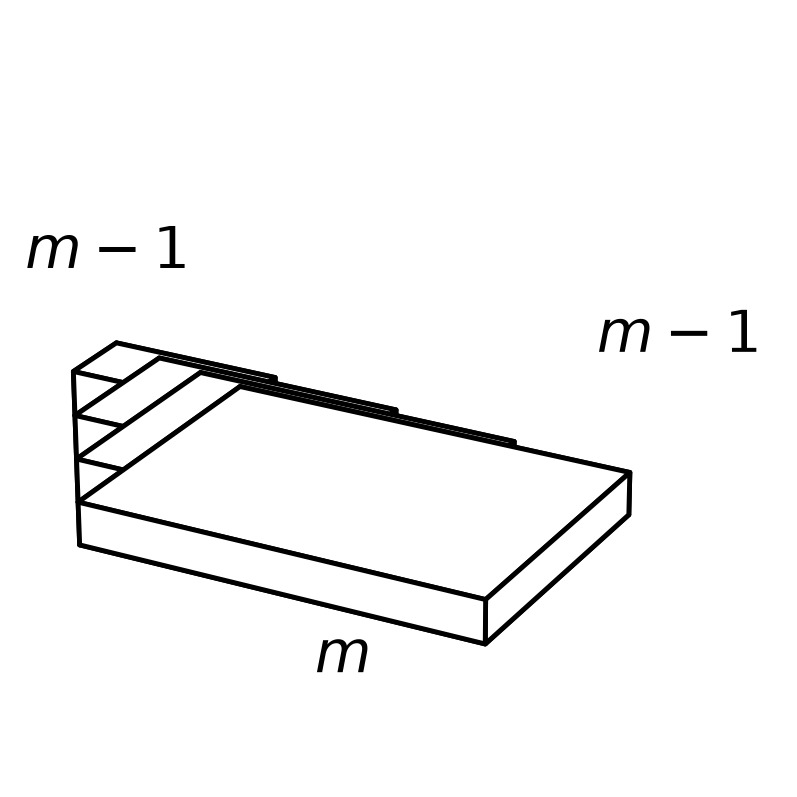
\includegraphics[width=0.46\linewidth]{../assets/figure-26-operation-left.png}
    \caption{左侧 Householder 更新所对应的运算量示意图。图中阶梯状实体的体积趋于 $\frac13m^3$。}
\end{figure}

当 $m\to\infty$ 时，体积趋于 $\frac13m^3$。每个元素需要 4 次浮点
运算，所以这个循环的工作量约为 $\frac43m^3$ 次浮点运算。

第二个内层循环从右侧施加 Householder 反射。第 $k$ 步通过形成最后
$m-k$ 列的线性组合来完成。这个循环比第一个循环工作量更大，因为
没有可以忽略的零；被操作的每一列的全部 $m$ 个元素都要计算，因此
对固定 $k$ 共涉及 $m(m-k)$ 个元素。几何示意如下：

\begin{figure}[H]
    \centering
    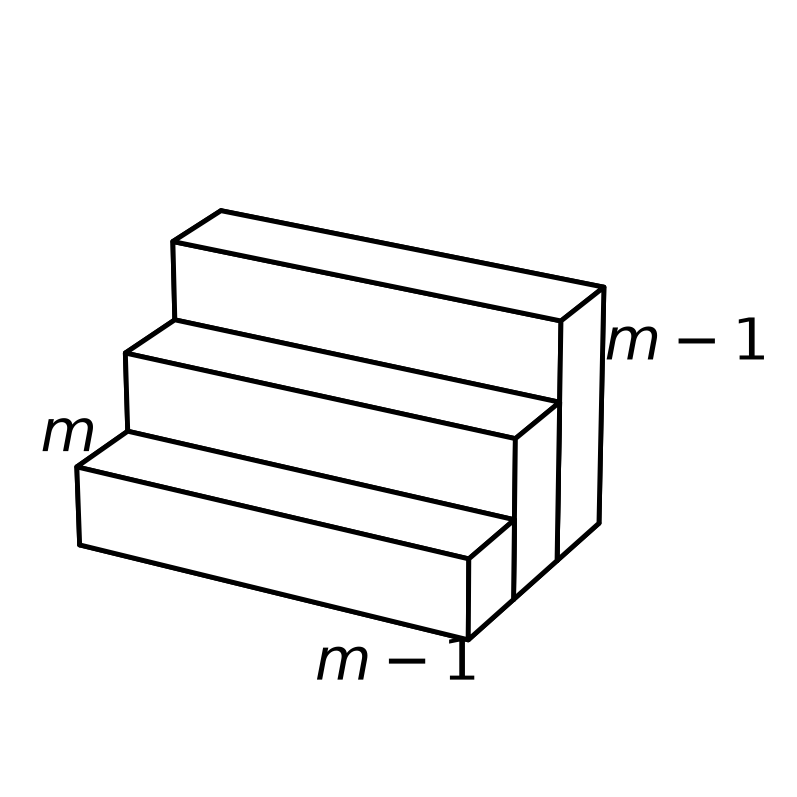
\includegraphics[width=0.46\linewidth]{../assets/figure-26-operation-right.png}
    \caption{右侧 Householder 更新所对应的运算量示意图。图中阶梯状实体的体积趋于 $\frac12m^3$。}
\end{figure}

当 $m\to\infty$ 时，体积趋于 $\frac12m^3$，所以每个元素需要
4 次浮点运算时，这个循环需要约 $2m^3$ 次浮点运算。

两部分相加，一个 $m\times m$ 矩阵进行酉约化、化为 Hessenberg 形式
的总工作量为
\begin{equation}
 \text{Hessenberg 约化的工作量}\sim\frac{10}{3}m^3\ \text{flops}.
\tag{26.1}
\end{equation}

\section*{Hermitian 情形：化为三对角形式}

如果 $A$ 是 Hermitian 矩阵，上述算法会把 $A$ 约化为三对角形式
（至少在没有舍入误差时如此）。原因很简单：$A$ 是 Hermitian，
$Q^*AQ$ 仍然是 Hermitian，而任意 Hermitian Hessenberg 矩阵都是
三对角矩阵。

由于现在行和列中都会引入零，因此可以忽略这些额外的零，进一步节省
运算。经过这种优化，右侧 Householder 反射的代价与左侧反射一样低，
右侧反射的总成本从 $2m^3$ 降为 $\frac43m^3$。此时相加的是两个
金字塔，而不是一个金字塔和一个棱柱，总运算量降为 $\frac83m^3$。

不过，这一节省只利用了稀疏性，而没有利用对称性。事实上，在计算的
每个阶段，被操作的矩阵都是 Hermitian 的。再利用这个结构还可以节省
一个因子 2，得到
\begin{equation}
 \text{三对角约化的工作量}\sim\frac43m^3\ \text{flops}.
\tag{26.2}
\end{equation}
实现细节不在此处给出。

\section*{稳定性}

和 QR 分解的 Householder 算法一样，刚才描述的算法是向后稳定的。
回忆定理 16.1：对任意 $A\in\mathbb{C}^{m\times n}$，QR 分解的
Householder 算法计算出的反射向量等价于一个隐式的、精确酉的因子
$\widetilde Q$，以及一个显式的上三角因子 $\widetilde R$，满足
\[
 \widetilde Q\widetilde R=A+\delta A,\qquad
 \frac{\|\delta A\|}{\|A\|}=O(\epsmach).
\]

算法 26.1 也可以建立同样的误差估计。令 $\widetilde H$ 表示浮点
运算中实际计算出的 Hessenberg 矩阵；令 $\widetilde Q$ 表示与浮点
计算出的反射向量相对应的、精确酉的矩阵。可以证明下述结果。

\paragraph{定理 26.1.}
设矩阵 $A\in\mathbb{C}^{m\times m}$ 的 Hessenberg 约化
$A=QHQ^*$ 由算法 26.1 在满足公理 (13.5) 和 (13.7) 的计算机上完成，
并按上面的方式定义计算因子 $\widetilde Q$ 和 $\widetilde H$。则存在
$\delta A\in\mathbb{C}^{m\times m}$，使得
\begin{equation}
 \widetilde Q\widetilde H\widetilde Q^*
 =A+\delta A,\qquad
 \frac{\|\delta A\|}{\|A\|}=O(\epsmach).
\tag{26.3}
\end{equation}

\section*{习题}

\paragraph{26.1.}
定理 26.1 及其后面各讲中的类似定理表明，我们可以数值计算 $A$ 的
特征值 $\{\widetilde\lambda_k\}$，并且这些数值正好是矩阵
$A+\delta A$ 的精确特征值，其中
$\|\delta A\|/\|A\|=O(\epsmach)$。这是否意味着它们接近 $A$ 的精确
特征值 $\{\lambda_k\}$？这是特征值扰动理论的问题。

可以用几何方式处理这类问题。给定
$A\in\mathbb{C}^{m\times m}$，其谱为 $\Lambda(A)\subset\mathbb{C}$，
以及 $\epsilon>0$，定义 $A$ 的 2-范数 $\epsilon$-伪谱
$\Lambda_\epsilon(A)$ 为满足以下任一条件的复数 $z$ 的集合：
\begin{enumerate}[label=(\roman*)]
  \item $z$ 是某个 $A+\delta A$ 的特征值，其中
  $\|\delta A\|_2\le\epsilon$；
  \item 存在 $u\in\mathbb{C}^m$，使
  $\|(A-zI)u\|_2\le\epsilon$ 且 $\|u\|_2=1$；
  \item $\sigma_m(zI-A)\le\epsilon$；
  \item $\|(zI-A)^{-1}\|_2\ge\epsilon^{-1}$。
\end{enumerate}
条件 (iv) 中的矩阵 $(zI-A)^{-1}$ 称为 $A$ 在 $z$ 处的预解算子
（resolvent）；如果 $z$ 是 $A$ 的特征值，约定
$\|(zI-A)^{-1}\|_2=\infty$。条件 (iii) 中的 $\sigma_m$ 表示最小
奇异值。证明条件 (i)--(iv) 等价。

\paragraph{26.2.}
设 $A$ 是一个 $32\times32$ 矩阵：主对角线上的条目为 $-1$，第一条
和第二条超对角线上的条目为 1，其余条目为 0。

\begin{enumerate}[label=(\alph*)]
  \item 使用 MATLAB 或其他软件系统中内置的 SVD 算法以及等高线绘图
  软件，绘制 $A$ 在
  \[
  \epsilon=10^{-1},10^{-2},\ldots,10^{-8}
  \]
  时的 2-范数 $\epsilon$-伪谱边界。
  \item 对 $0\le t\le50$ 绘制 $\|e^{tA}\|_2$ 关于 $t$ 的半对数图。
  在最终衰减出现以前，曲线的初始增长率是多少？能否把它与伪谱图
  联系起来？（与习题 24.3 对照。）
\end{enumerate}

\paragraph{26.3.}
特征值扰动理论中最著名的结果之一是 Bauer--Fike 定理。设
$A\in\mathbb{C}^{m\times m}$ 可对角化，即
$A=V\Lambda V^{-1}$，并令 $\delta A\in\mathbb{C}^{m\times m}$ 任意。
那么 $A+\delta A$ 的每个特征值，至少落在复平面上 $m$ 个圆盘中的
一个内；这些圆盘的圆心是 $A$ 的特征值，半径为
$\kappa(V)\|\delta A\|_2$，其中 $\kappa$ 是 2-范数条件数。
（与习题 24.2 对照。）

\begin{enumerate}[label=(\alph*)]
  \item 利用习题 26.1 中条件 (i) 和 (iv) 的等价性，证明 Bauer--Fike
  定理。
  \item 假设 $A$ 是正规矩阵。证明：对 $A+\delta A$ 的每个特征值
  $\widetilde\lambda_j$，都存在 $A$ 的一个特征值 $\lambda_j$，使得
                   \begin{equation}
   |\widetilde\lambda_j-\lambda_j|\le\|\delta A\|_2.
   \tag{26.4}
  \end{equation}
\end{enumerate}

\end{document}
